\documentclass{article}
\usepackage{graphicx}
\usepackage{tikz}
\usetikzlibrary{positioning,fit}
\newcommand\toolav[1]{toolA}
\begin{document}
\begin{figure}[hbt]
    \resizebox{\textwidth}{!}{%
    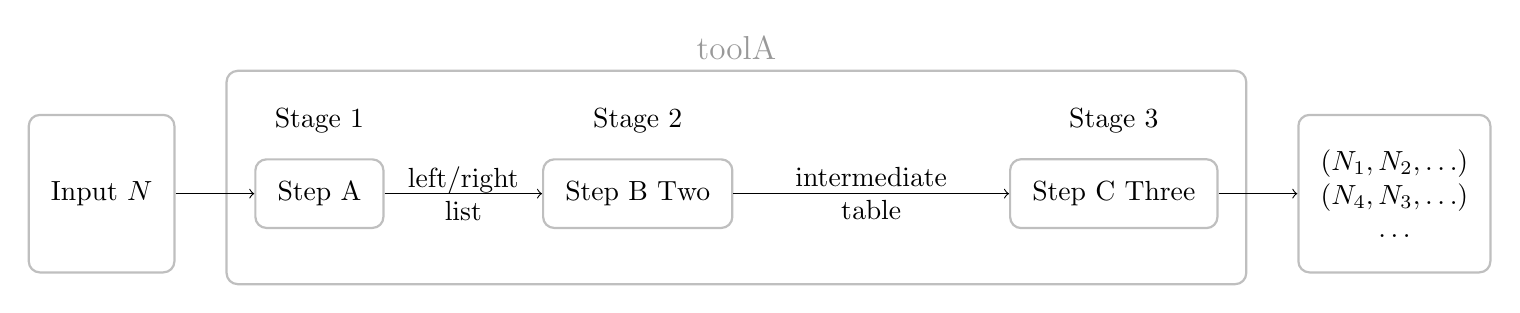
\begin{tikzpicture}[
         stage/.style={draw=gray!50, rounded corners, inner sep = 8pt, thick},
    ]

        \node[stage, minimum height=2cm] (inputbox) { Input $N$};

        \node[stage, right=of inputbox] (stepone) { Step A };
        \node[above=2mm of stepone] (l1) {Stage 1};

        \node[stage, right=2cm of stepone] (steptwo) { Step B Two };
        \node[above=2mm of steptwo] (l2) {Stage 2};

        \node[stage, right=3.5cm of steptwo] (stepthree) { Step C Three };
        \node[above=2mm of stepthree] (l3) {Stage 3};

        \node[stage, right=of stepthree, minimum height=2cm, align=center] (output) { $(N_1,N_2,\dots)$\\$(N_4,N_3,\dots)$\\$\dots$ };

        \node[below=1mm of stepone] (spacer) {};

        \node [stage, inner sep=10pt, fit={(stepone) (steptwo) (stepthree) (l1) (l2) (l3) (spacer)}] (toola) {};


        \node[above=0mm of toola, gray!80] {\large \toolav{0}};

        \draw[->] (inputbox) -- (stepone);
        \draw[->] (stepone) -- (steptwo) node [midway, align=center] {left/right\\list};
        \draw[->] (steptwo) -- (stepthree) node [midway, align=center] {intermediate\\table};
        \draw[->] (stepthree) -- (output);

    \end{tikzpicture}
    }
\end{figure}
\gdef\SatexReachedEnd{}
\end{document}
